%!TEX root = Nanomat.tex
\ctitle{Superkritiske fluider}
\paragraph{Definisjon: superkritisk fluid} I området i et $p,T$-fasediagram som er ``forbi'' et det superkritiske punktet $(T_c,p_c)$ har materialet egenskaper som verken er helt som væsker eller helt som gasser, og kalles et \idx{superkritisk fluid} (se Figur~\ref{fig:carbondioxide}). Som jeg ikke helt har fått til å uttrykke i figuren, så er det en glidende overgang mellom gass, superkritisk fluid og væske. 
\begin{figure}[H]
	\bmd\centering
	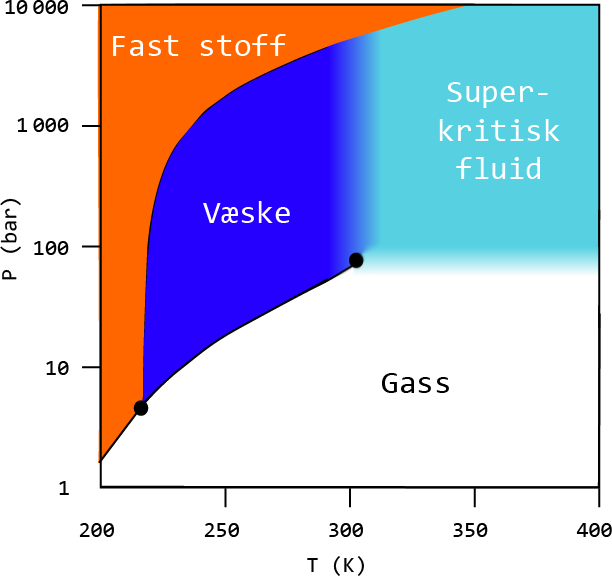
\includegraphics[width=0.9\linewidth]{carbondioxide.png}
	\caption{$p,T$-fasediagram for karbondioksid. En endring fra gass til væske, gass til fast stoff eller væske til fast stoff er markert med brå fargeendringer for å reflektere at disse overgangene medfører en brå endring av tetthet og andre egenskaper. Endringene fra væske til superkritisk fluid, og fra gass til superkritisk fluid, er gradert fordi disse faseendringene er kontinuerlige. Det markerte punktet nede til venstre er trippelpunktet, punktet oppe til høyre er det kritiske punktet.}
	\label{fig:carbondioxide}
\emd\end{figure}

\cstitle{Egenskaper for superkritiske fluider}
Egenskapene til et superkritisk fluid endrer seg raskt i området rundt det kritiske punktet.

\paragraph{Tetthet} Tettheten til et superkritisk fluid er gjerne nærmere en væske enn en gass, og tettheten varierer raskt rundt det kritiske punktet.

\paragraph{Løselighet} Løseligheten til materialer i et superkritisk løsemiddel er gitt ved løsemiddelets \emph{oppløsningsevne} $\delta_{\text{f}}$:
\begin{equation}
	\delta_{\text{f}} = 1.25\sqrt{P_c}\frac{\rho_{\text{s.kr. fluid}}}{\rho_{\text{væske}}},
\end{equation}
der $P_c$ er trykket i det superkritiske fluidet og $\rho$ er tettheter ($\rho_{\text{væske}}$ er tettheten som fluidet ville hatt om det var i væsketilstand). $\rho_{\text{s.kr. fluid}}$ avhenger naturligvis av trykk og temperatur.

\paragraph{Viskositet} Viskositeten til et superkritisk fluid er mellom en hundredel og en tidel av viskositeten til en væske, men fortsatt høyere enn viskositeten til en gass. I nærheten av det kritiske punktet øker viskositeten veldig raskt med økende trykk.

\paragraph{Diffusjon} Transportegenskapene til et superkritisk fluid er mellom egenskapene til en gass og egenskapene til en væske. Diffusjonskonstanten har en størrelsesorden halvveis mellom den for en gass og den for en væske. Den øker når trykket faller eller temperaturen stiger.

Hvis man antar at diffusjon er et resultat av Brownske bevegelser, og at hver partikkel i løsning er en kule med radius $r$, så kan man finne diffusjonskonstanten via Stokes-Einstein-ligningen
\begin{equation}
	D=\frac{RT}{6N\pi\eta r},
\end{equation}
der $\eta$ er viskositet. 

For å finne diffusjonskonstanten kan vi i enkelte tilfeller måle den midlere frie banen til partiklene (for eksempel med mikroskop) og bruke den statistiske relasjonen
\begin{equation}
	\overline{x} = \sqrt{2Dt}.
\end{equation}

\paragraph{Termisk konduktivitet} I superkritiske fluider observerer man en ``fjerde'' mekanisme for varmetransport (sammen med varmeledning, konveksjon og varmestråling) dersom man varmer opp én vegg i beholderen der man har det superkritiske fluidet. Mekanismen man ser for seg er at laget som er i kontakt med den varme veggen varmes opp og utvider seg, og dermed komprimerer resten av fluidet, som så varmes opp veldig raskt. Dette beskrives som en ``piston effect'' fordi fluidet varmes opp på samme måte som gass gjør når det komprimeres med et stempel.
\vfill
\cstitle{Bruksområder for superkritiske fluider}

Det er to klasser av brukesområder for superkritiske fluider. Den ene er rensing og ekstrahering, den andre er syntese.

\paragraph{Rensing og ekstrahering med superkritiske fluider} Siden oppløsningsevnen til superkritiske fluider varierer med både trykk og temperatur (i motsetning til bare temperatur, som er tilfellet med væsker), er de nyttige for ekstrahering. Et godt eksempel er bruk av superkritisk \ce{CO2} for å ekstrahere koffein fra kaffebønner. Prosessen er som følger:
\begin{enumerate}
	\item Kaffebønner og \ce{CO2} puttes i et kammer med trykk og temperatur som gjør \ce{CO2} superkritisk. Den superkritiske væsken ekstraherer koffein fra bønnene.
	\item Trykket i kammeret senkes til det er under det superkritiske punktet, slik at \ce{CO2} blir en gass. Dette gjør at løseligheten til koffein faller raskt, og koffein felles ut.
\end{enumerate}

\cstitle{Syntese med superkritiske fluider}
Egenskapene til superkritiske fluider kan brukes for å syntetisere nanomaterialer. Dette kan oppnås både med fysiske prosesser (der kun fysiske størrelser som temperatur og trykk endres) og kjemiske prosesser (der fluidet brukes som reaksjonsmedium).

\paragraph{Fysiske metoder - Rapid expansion of a supercritical solution (RESS)} Dette er den viktigste fysiske metoden å få med seg. Materialet løses først opp i det superkritiske fluidet. Deretter senkes trykket raskt, slik at løseligheten faller raskt og materialet felles ut. Å ``senke trykket raskt'' kan være så enkelt som å åpne en ventil til et annet kammer med lavere trykk. Dette viser seg å gi partikler med en veldig smal størrelsesfordeling. Man kan få forskjellige former og størrelser på partiklene avhengig av eksperimentelle betingelser.

Et krav for denne metoden er at produktet som skal lages, i utgangspunktet må være løselig i det superkritiske fluidet.

\paragraph{Fysiske metoder - Physical Process Without Expansion} Dette er å bruke det superkritiske fluidet til å lage komposittmaterialer, ved å ``spre det oppløste materialet utover'' en matrise. Superkritiske fluider fungerer bra til dette fordi de har lav viskositet og høy diffusjonskonstant, som hjelper det oppløste stoffet med å komme inn i matrisen. Det er ikke så veldig mye man har klart å lage med denne prosessen.

\paragraph{Fysiske metoder - Antisolvent Process with Supercritical Fluids} Dette er også en ting som det står om i Cushing. Jeg håper det ikke er viktig.

\paragraph{Kjemiske metoder - syntese av nanotråder} I kjemiske metoder brukes det superkritiske fluidet som reaksjonsmedium. Et eksempel på dette er vekst av silisium-nanotråder på gullpartikler: man har gullpartikler i en løsning av superkritisk heksan, og en silisium-precursor (difenylsilan) som raskt brytes ned til silisiumatomer. Når det er nok silisium i forhold til gull, løses silisium opp i gullpartiklene og danner en legering. Etter hvert som konsentrasjonen av silisium i gullpartiklene blir større, vil silisium frastøtes mot overflaten. Etter hvert som det kommer nye silisiumatomer til overflaten, dytter de ut silisiumatomene overfor og danner en nanotråd av silisium som vokser ut av gullpartikkelen.

\paragraph{Kjemiske metoder - SCF i micellesystemer} En annen kjemisk metode er bruk av superkritiske fluider i \emph{micellesystemer} med reverserte miceller. Mekanismen er den samme som i kapittel 18, men kinetikken påvirkes av at diffusjonskonstanten er opp til 100 ganger større enn i væske. I tillegg kan man med superkritiske fluider bruke trykk til å påvirke størrelsen til partiklene. Økt trykk fører til et økt vanninnhold i micellene, slik at micellene blir større. % Noe med trykkavlastning her også